\documentclass[12pt, a4paper]{report}
\usepackage{graphicx} %LaTeX package to import graphics
\usepackage[shortlabels]{enumitem}
\usepackage{geometry}
\usepackage{xcolor}
\geometry{lmargin=30mm}
\usepackage[export]{adjustbox}
\usepackage{titlesec}
\usepackage{float}
\titleformat{\chapter}{\normalfont\huge}{\thechapter}{20pt}{\huge\bf}
\graphicspath{{images/}} %configuring the graphicx package
\title{Practica 2}
\author{Javier Izquierdo Hernández}
\date{\today}
\begin{document}
	\begin{titlepage}
		\centering
		{
\includegraphics[width=0.3\textwidth]{logo}\par}
		\vspace{1cm}
		{\bfseries\LARGE Universidad Rey Juan Carlos \par}
		\vspace{1cm}
		{\scshape\Large E.T.S. Ingeniería de Telecomunicación \par}
		\vspace{3cm}
		{\scshape\Huge Redes de Ordenadores para Robots y Máquinas Inteligentes \par}
		\vspace{3cm}
		{\itshape\Large Práctica 2 \par}
		\vfill
		{\Large Autor: \par}
		{\Large Javier Izquierdo Hernández \par}
		\vfill
		{\Large \today \par}
	\end{titlepage}

\newpage
\renewcommand{\contentsname}{Contenidos}
\tableofcontents
\newpage

\chapter{Configuración básica de un servidor de DHCP}
Descomprime el fichero lab-DHCP.tgz. Arranca NetGUI y en el menú, elige File → Open y selecciona la
carpeta lab-DHCP en la que has descomprimido el escenario. Verás aparecer la red de la figura 1.\\

\begin{figure}[h]
	\centering
	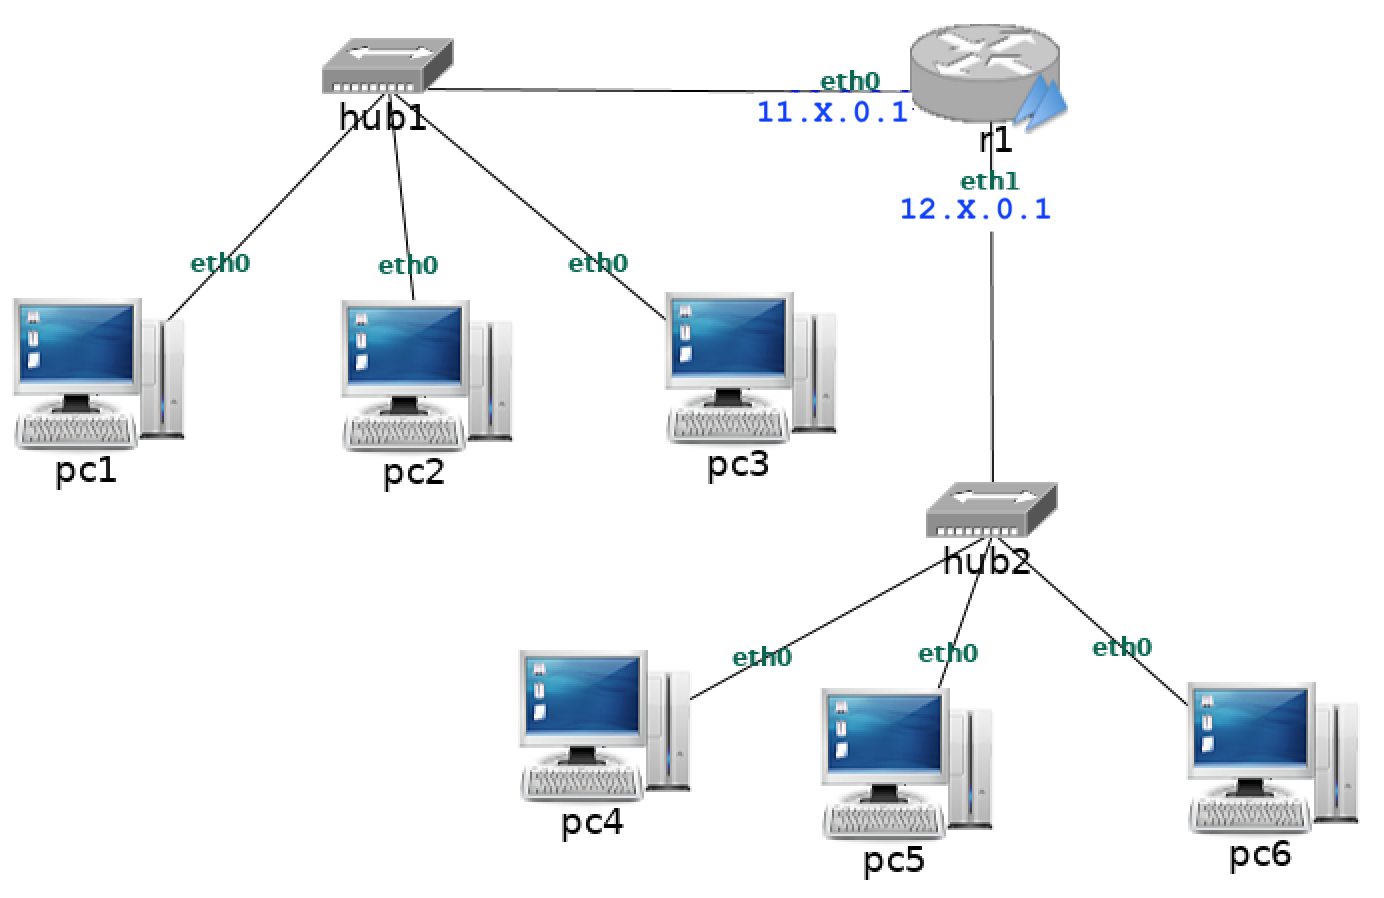
\includegraphics[width=0.7\textwidth]{enunciado_1}
	\caption{Escenario lab-DHCP}
\end{figure}
Arranca \textbf{exclusivamente} r1.\\

Verás que r1 es un router conectado a las dos subredes de la figura, por lo que lo utilizaremos para alojar
al servidor de DHCP de todas las máquinas de ambas subredes. Recuerda que si un servidor DHCP no está en
la misma subred que algunos de sus clientes será necesario configurar un repetidor (relay) DHCP que reenvíe
los mensajes entre clientes y servidores de distintas subredes.
\begin{enumerate}
	\item Configura en r1 el fichero \textcolor{blue}{/etc/default/dhcp3-server} para que r1 active el protocolo DHCP por sus
	dos interfaces.\\
	\begin{center}
		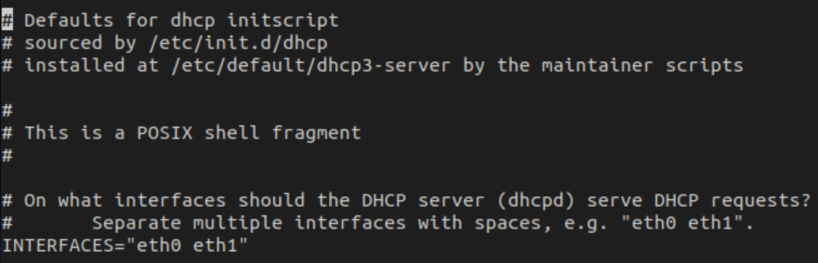
\includegraphics[width=0.5\textwidth]{ej1_1}
	\end{center}
	\item Configura en r1 el fichero \textcolor{blue}{/etc/dhcp3/dhcpd.conf} asignar 2 rangos de direcciones dinámicas a las dos
	subredes a las que r1 está conectado. Asegúrate de dejar fuera de cada pool de direcciones dinámicas
	las direcciones IPs de r1, y algunas más adicionales para poder asignarlas de forma fija a alguna de las
	máquinas. Incluye también en la configuración de la subred un \textit{router} por defecto.\\
	No arranques todavía el servidor de DHCP.\\
	\begin{center}
		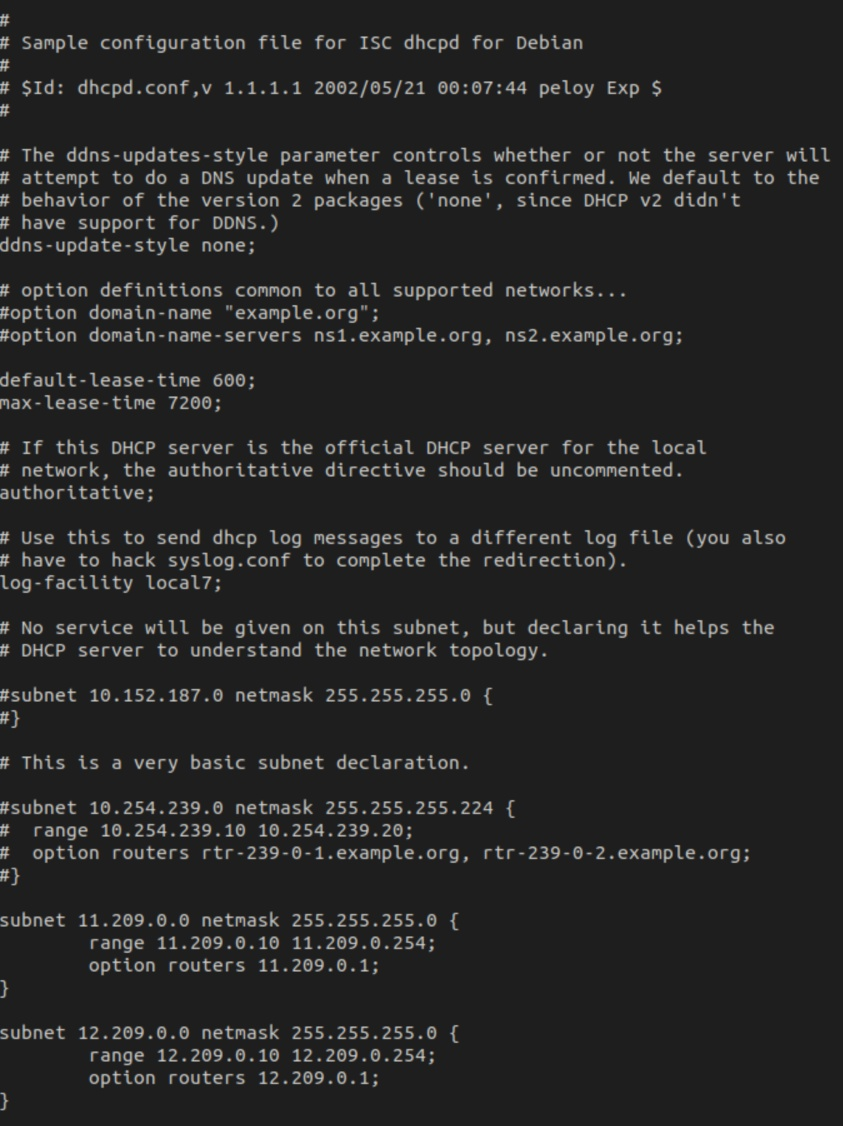
\includegraphics[width=0.6\textwidth]{ej2_1}
	\end{center}
\end{enumerate}

\chapter{Configuración inicial de clientes de DHCP}
\begin{enumerate}
	\item Asegúrate de que aún no está arrancado el servidor de DHCP en r1.\\
	Inicia una captura con tcpdump en la interfaz eth0 (\textcolor{blue}{dhcp-1.cap}).\\
	Arranca pc1 y pc4. Verás en sus ventanas de terminal que están intentando obtener una dirección IP
	por DHCP, pero el servidor aún no está arrancado.\\
	Espera unos minutos hasta que pc1 y pc4 desistan y completen el arranque. Comprueba qué direcciones
	IP tienen asignadas pc1 y pc4. Comprueba qué direcciones Ethernet tienen asignada pc1 y pc4 y anótalas.\\
	\begin{center}
		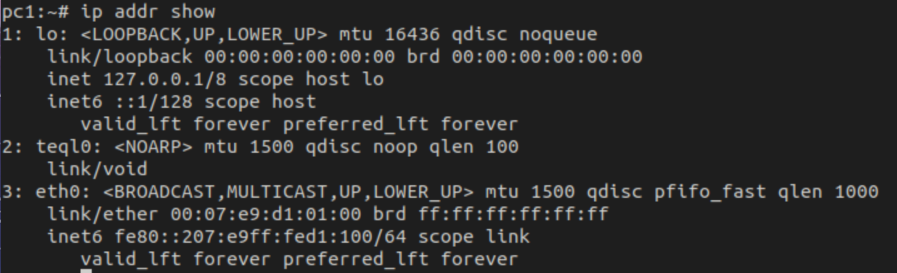
\includegraphics[width=0.6\textwidth]{ej1_1_2}
		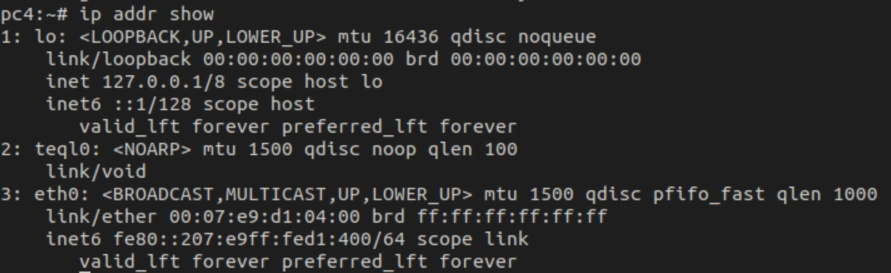
\includegraphics[width=0.6\textwidth]{ej1_2_2}
	\end{center}
	Comprueba en su fichero \textbf{/etc/network/interfaces} cómo pc1 tiene configurado que obtenga su dirección por DHCP.\\
	\begin{center}
		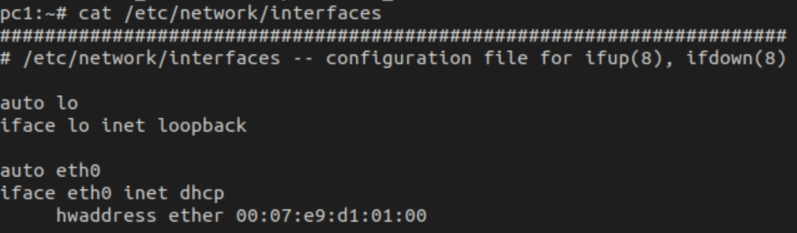
\includegraphics[width=0.6\textwidth]{ej1_3_2}
	\end{center}
	Interrumpe la captura y ábrela en wireshark. En la captura verás mensajes del protocolo ICMPv6 que
	son parte de la configuración de IPv6: estos mensajes no son objeto de estudio en esta práctica. Identifica
	en la captura los mensajes de DHCP que aparecen en ella.\\
	Son los mensajes señalados en azul.
	\begin{center}
		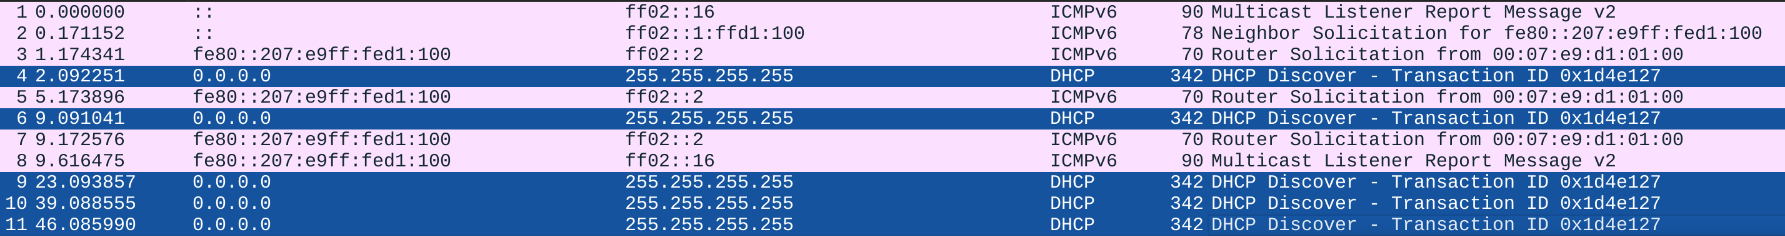
\includegraphics[width=\textwidth]{ej1_4_2}
	\end{center}
	Apaga las máquina pc1 y pc4.
	\item Configura en r1 el servidor de DHCP para que asigne una dirección fija a las máquinas pc1 y pc4. Utiliza
	las direcciones Ethernet de ambas máquinas que has anotado en el apartado anterior.\\
	\begin{center}
		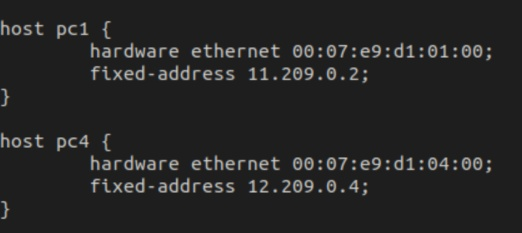
\includegraphics[width=0.6\textwidth]{ej2_2}
	\end{center}
	Arranca (en \textit{background}) en r1 una captura con tcpdump en la interfaz eth0 (\textcolor{blue}{dhcp-2.cap}).\\
	\textbf{Arranca ahora el servidor de DHCP} en r1.
	\item Arranca de nuevo pc1. Cuando termine de arrancar completamente, arranca también pc2. No interrumpas
	aún la captura en curso.
	\item Comprueba que tanto pc1 como pc2 han obtenido su dirección al arrancar.\\
	\begin{center}
		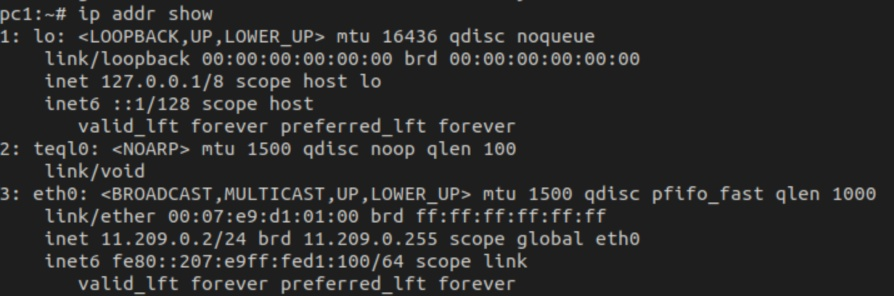
\includegraphics[width=0.6\textwidth]{ej4_1_2}
		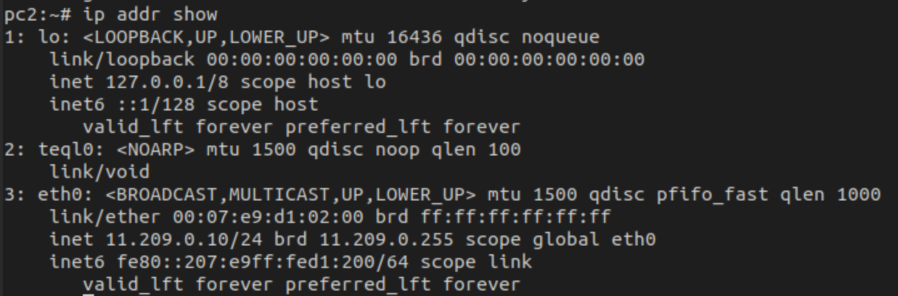
\includegraphics[width=0.6\textwidth]{ej4_2_2}
	\end{center}
	\item Si han pasado al menos 5 minutos desde que arrancaron pc1 y pc2, interrumpe la captura en curso.
	Reconoce en la captura las interacciones cliente–servidor explicadas en la parte teórica del tema. Responde
	a las siguientes cuestiones:
	\begin{enumerate}[a)]
		\item Localiza los mensajes pertenecientes a la transacción con la que se configura la dirección de pc1 y
		a la de pc2. ¿Cómo los distingues?\\
		
		Se pueden distinguir con las direcciones Ethernet, por las direcciones Ip sabiendo que la de pc1 acaba en .2 o también por el orden que hemos seguido para realizar la captura, siendo primero pc1 y luego pc2.
		\begin{figure}[!h]
			\centering
			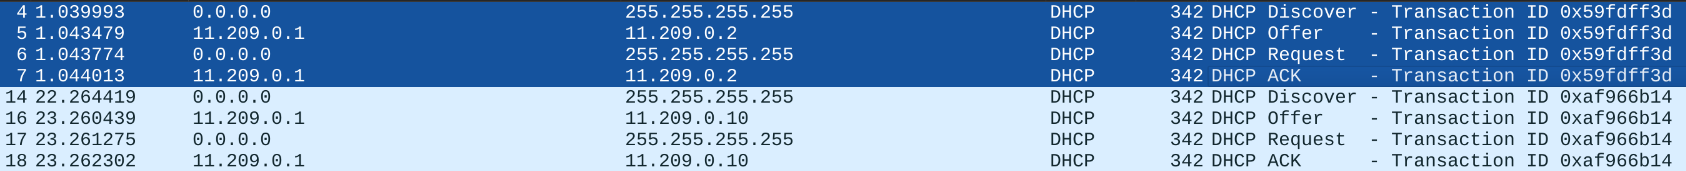
\includegraphics[width=\textwidth]{ej5_1_2}
		\end{figure}
		\item ¿Cuál es la dirección de destino Ethernet de los distintos mensajes que envía un cliente? ¿Y la
		dirección de destino IP? Observa en estos mensajes el valor de los 4 campos de direcciones IP de la
		cabecera DHCP.\\
		
		Esto solo lo voy a explicar para pc1, pero pc2 es equivalente.
		\begin{enumerate}
			\item Primer mensaje
			\begin{itemize}
				\item Ethernet destino: ff:ff:ff:ff:ff:ff Broadcast
				\item Ip destino: 255.255.255.255
				\item El valor de los 4 campos de direcciones Ip es 0.0.0.0
			\end{itemize}
			\item Segundo mensaje
			\begin{itemize}
				\item Ethernet destino: ff:ff:ff:ff:ff:ff Broadcast
				\item Ip destino: 255.255.255.255
				\item El valor de los 4 campos de direcciones Ip es 0.0.0.0
			\end{itemize}
		\end{enumerate}
		\item ¿Cuáles son las direcciones de destino Ethernet e IP de los distintos mensajes de respuesta que envía
		el servidor? Observa en estos mensajes el valor de los 4 campos de direcciones IP de la cabecera
		DHCP.\\
		
		Esto solo lo voy a explicar para los mensajes recibidos por pc1, pero para pc2 es equivalente.
		\begin{enumerate}
			\item Primer mensaje
			\begin{itemize}
				\item Ethernet destino: 00:07:e9:d1:01:00 (00:07:e9:d1:02:00 Pc2)
				\item Ip destino: 11.209.0.2 (11.209.0.10 Pc2)
				\item El valor de 3 campos de direcciones Ip es 0.0.0.0, excepto en el campo de \textit{Your (client) IP address} que es 11.209.0.2 (11.209.0.10 Pc2)
			\end{itemize}
			\item Segundo mensaje
			\begin{itemize}
				\item Ethernet destino: 00:07:e9:d1:01:00 (00:07:e9:d1:02:00 Pc2)
				\item Ip destino: 11.209.0.2 (11.209.0.10 Pc2)
				\item El valor de 3 campos de direcciones Ip es 0.0.0.0, excepto en el campo de \textit{Your (client) IP address} que es 11.209.0.2 (11.209.0.10 Pc2)
			\end{itemize}
		\end{enumerate}
		\item Localiza en los mensajes enviados por un cliente los parámetros de configuración solicitados, que
		deberán coincidir con lo especificado en el fichero de configuración del cliente DHCP.\\
		
		Como se puede ver en las imágenes inferiores los parámetros de configuración son iguales a los solicitados.
		\begin{figure}[!h]
			\centering
			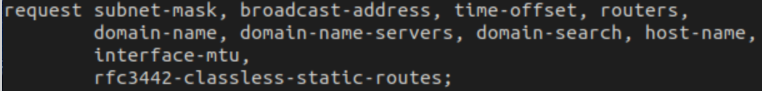
\includegraphics[width=0.7\textwidth]{ej5_4_2}
			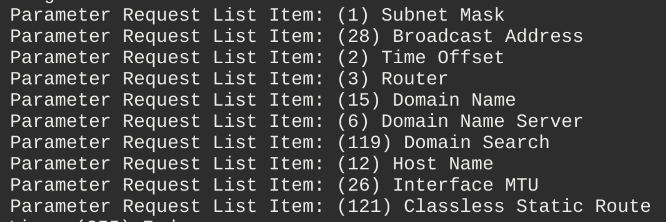
\includegraphics[width=0.7\textwidth]{ej5_5_2}
		\end{figure}
		\item ¿Se utiliza en esta implementación el flag de broadcast de DHCP? ¿Qué implicaciones tiene esto?\\
		
		No se utiliza el flag de Broadcast, porque en esta implementación los pc tienen la capacidad de recibir datagramas a una dirección Ip que no tienen asignada.
		\item Observa el proceso de configuración de pc1. ¿Chequea el servidor de alguna manera que la IP que
		ofrecerá a pc1 está libre? ¿Por qué?\\
		
		No, porque hemos configurado en r1 una dirección estática para pc1 y esta siempre será de pc1.
		\item Observa el proceso de configuración de pc2. ¿Chequea el servidor de alguna manera que la IP que
		ofrecerá a pc2 está libre? ¿Por qué?\\
		
		Si que chequea que la Ip está libre, ya que pc2 al contrario de pc1 no tiene ninguna Ip estática configurada, por lo tanto tiene que coger una Ip de la pool de direcciones dinámicas de r1.
		\item En esta implementación, una vez asignada la IP a un cliente, ¿comprueba el servidor que el cliente
		ha activado dicha IP? ¿En qué casos? ¿Cómo lo hace?\\
		
		Si que lo hace, pero solo en los casos en que la Ip dada es parte de la pool de direcciones Ip dinámicas como con pc2, y lo hace haciendo un ping a la dirección Ip que acaba de asignar.
		\item En esta implementación, una vez asignada la IP a un cliente, ¿comprueba el cliente que la IP
		realmente está disponible? ¿Por qué crees que actúa así?\\
		
		El cliente no comprueba que la Ip esté disponible, ya que este confía en que el servidor se la ha asignado de forma correcta.
		\item Mira la tabla de rutas de pc1 y de pc2. ¿Se ha activado alguna ruta como consecuencia de DHCP?\\
		
		Si, cuando consigue la Ip gracias a DHCP se activan las rutas que se ven en la imagen inferior.
		\begin{center}
			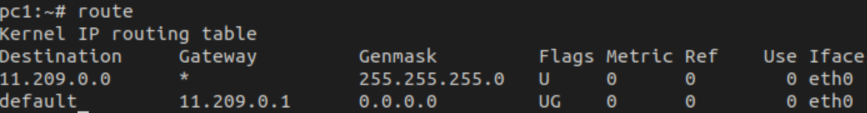
\includegraphics[width=0.6\textwidth]{ej5_2_2}
			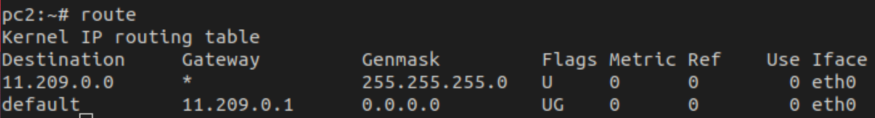
\includegraphics[width=0.6\textwidth]{ej5_3_2}
		\end{center}
	\end{enumerate}
\end{enumerate}

\chapter{Renovación de concesiones}
\begin{enumerate}
	\item El servidor escribe en el fichero \textcolor{blue}{/var/lib/dhcp3/dhcpd.leases} la información sobre las concesiones que
	realiza, para poder recuperarla tras reinicios o caídas. Consulta este fichero en r1 para ver su contenido.
	¿Por qué sólo aparece información sobre una de las dos IP que ha otorgado el servidor? NOTA: Ten en
	cuenta que en el fichero de concesiones la hora se guarda en formato UTC (1h menos que la hora CET,
	2h menos que la hora CEST).\\
	
	Solo aparece la IP que cede a pc2, ya que la que cede a pc1 es fija.
	\begin{center}
		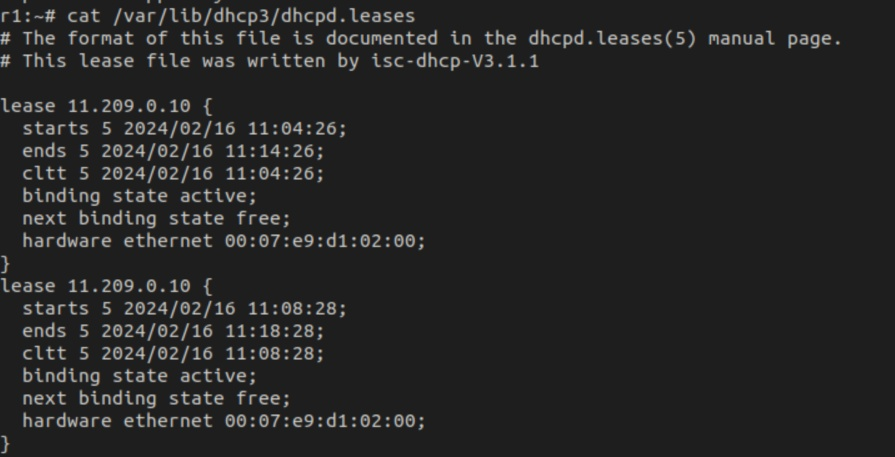
\includegraphics[width=0.6\textwidth]{ej1_3}
	\end{center}
	\item El cliente escribe en el fichero \textcolor{blue}{/var/lib/dhcp3/dhclient.eth0.leases} la información sobre la concesión
	que ha recibido por dicha interfaz. Estudia su contenido. ¿Por qué pc1 tiene esta información sobre su
	concesión y r1 no? Observa cómo aparecen anotadas en este fichero las horas de renovación, rebinding y
	expiración.\\
	
	Porque pc1 no conoce como maneja las Ip r1, por lo tanto para pc1 es como si se le hubiera asignado una Ip dinámica. Mientras que r1 si que sabe que la Ip de pc1 siempre será de pc1 ya que es fija, por lo que no hace falta tener la información sobre su concesión.
	\begin{figure}[H] % Do not use only [h] in real documents.
		\begin{minipage}[t]{.45\linewidth}
			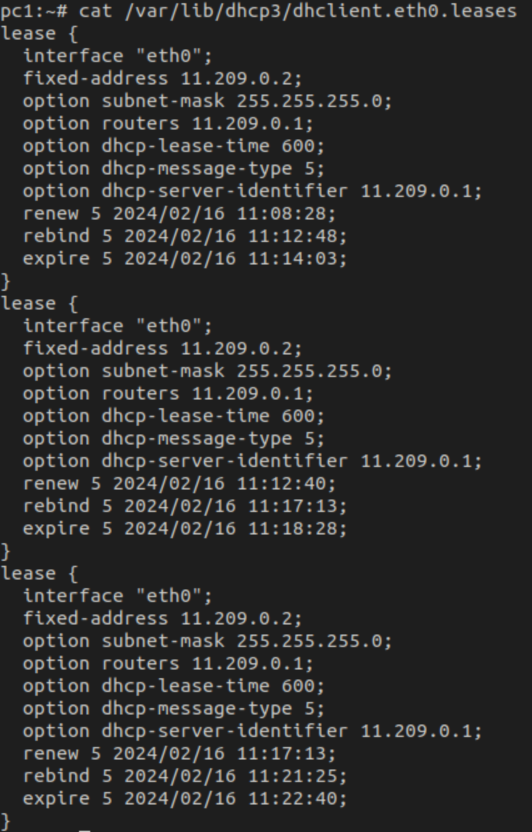
\includegraphics[width=\linewidth]{ej2_1_3}
		\end{minipage}\hfill
		\begin{minipage}[b]{.45\linewidth}
			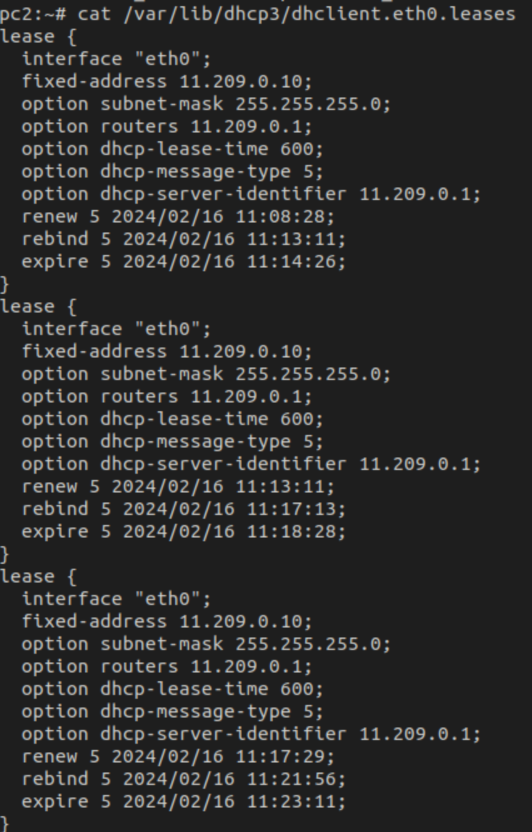
\includegraphics[width=\linewidth]{ej2_2_3}
		\end{minipage}
	\end{figure}
	\item Localiza en la captura realizada en el apartado anterior los mensajes correspondientes a la renovación
	de la concesión. Localiza en los primeros mensajes exactamente en cuál de ellos figura el tiempo T de
	la concesión. Dado ese valor ¿es adecuado el momento de hacer la renovación? Verás que pc1 y pc2 no
	calculan exactamente igual la hora de renovación y \textit{rebind}, ¿por qué crees que ocurre esto?\\
	
	El tiempo de la concesión es de 600 segundos o 10 minutos como también se aprecia viendo en las imágenes de arriba el incremento del renew time y del expire time.\\
	Con este valor se ve que el momento para hacer la renovación es el adecuado, ya que es aprox. 5 minutos.\\
	Luego en cuanto a la diferencia de los horarios de pc1 y pc2 se deberá principalmente al tiempo en el que hallan mandado su discovery.
	\item Empieza una nueva captura en r1-eth0 (\textcolor{blue}{dhcp-3.cap}). Reinicia pc2. Cuando termine de rearrancar por
	completo, interrumpe la captura y estúdiala:
	\begin{enumerate}[a)]
		\item ¿Hace algo DHCP en pc2 en el momento de apagarse?\\
		
		Sí, manda un mensaje de Release para que r1 sepa que la ip no está en uso.
		\item Señala las diferencias que se producen en el proceso de obtención de la dirección de pc2 con respecto
		a la captura anterior, incluyendo las comprobaciones que hacen servidor y cliente, y explícalas.\\
		
		Las dos diferencias más importantes son que en la primera captura para comprobar que la Ip no está está ocupada el router manda un datagrama Arp mientras que en la segunda r1 manda un ping a la Ip. Luego la otra es que en la primera captura r1 si comprueba que la Ip ha sido ocupada mientras que en la segunda no lo hace.
		\begin{figure}[!h]
			\centering
			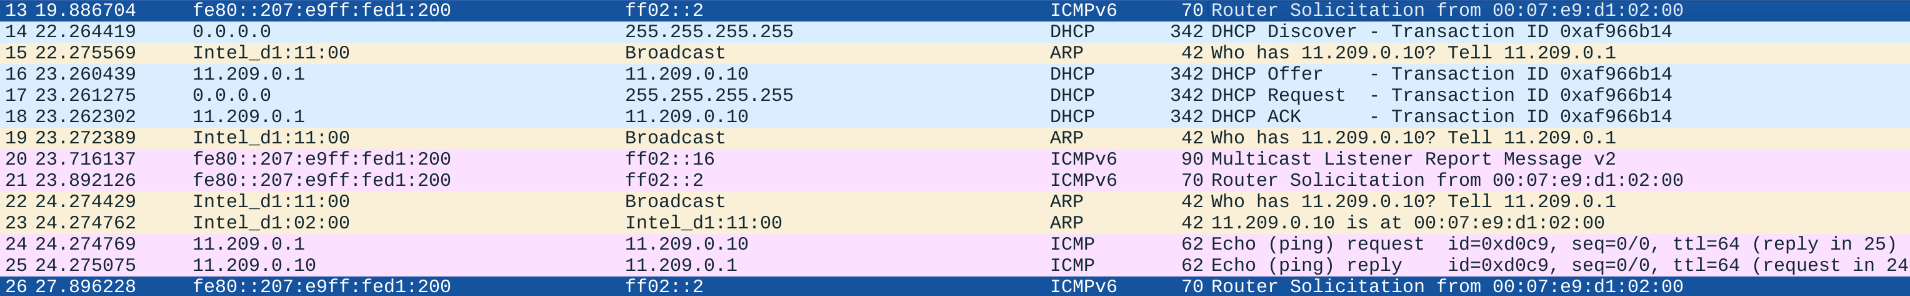
\includegraphics[width=\textwidth]{ej4_1_3}
			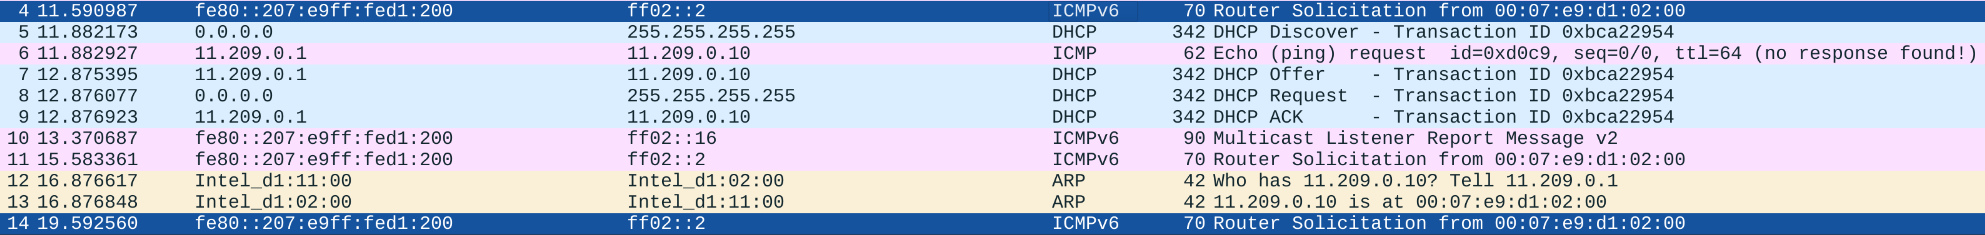
\includegraphics[width=\textwidth]{ej4_2_3}
		\end{figure}
	\end{enumerate}
\end{enumerate}

\chapter{Renovación de concesiones}
\begin{enumerate}
	\item Comprueba en el fichero de \textit{leases} de pc1 y pc2 a qué hora les toca la próxima renovación. Empieza
	(en \textit{background}) una nueva captura en r1-eth0 (\textcolor{blue}{dhcp-4.cap}). Interrumpe la ejecución del servidor de
	DHCP de r1.	\\
	\begin{figure}[!h]
		\centering
		\begin{minipage}[t]{.45\linewidth}
			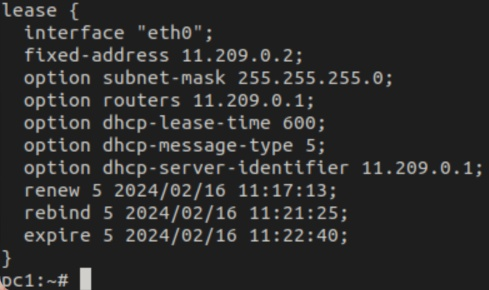
\includegraphics[width=\linewidth]{ej1_1_4}
		\end{minipage}\hfill
		\begin{minipage}[b]{.45\linewidth}
			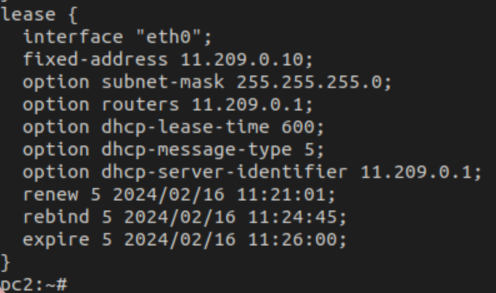
\includegraphics[width=\linewidth]{ej1_2_4}
		\end{minipage}
	\end{figure}
	\item Espera hasta que se rebase en 10 minutos la hora de expiración para interrumpir la captura. Observa
	qué ocurre tras alcanzarse dicha hora de expiración en pc1 y pc2 con respecto a sus direcciones IP.	\\
	
	Ambos pc pierden sus direcciones IP en eth0.\\
	
	\begin{tabular}{ll}
		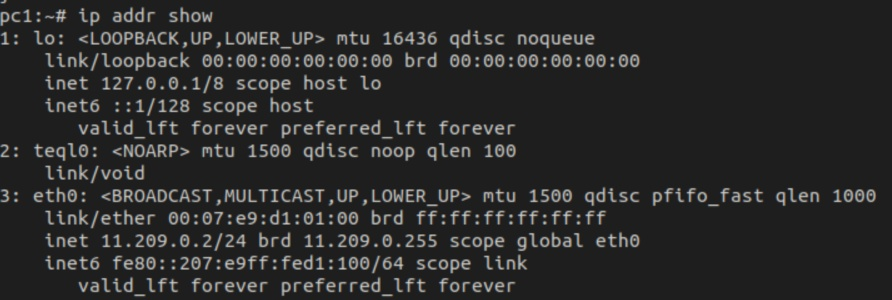
\includegraphics[width=0.4\textwidth]{ej2_1_4}&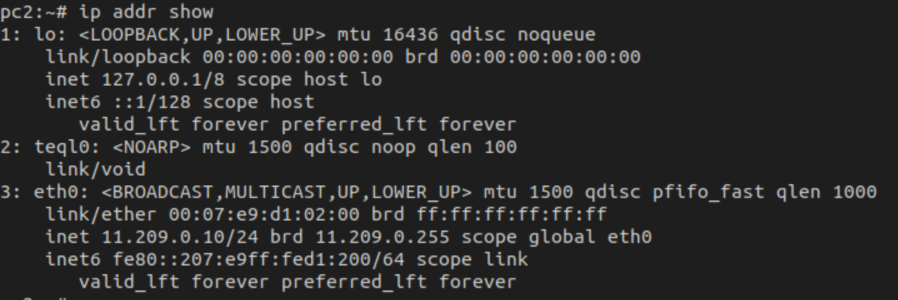
\includegraphics[width=0.4\textwidth]{ej2_2_4}\\
		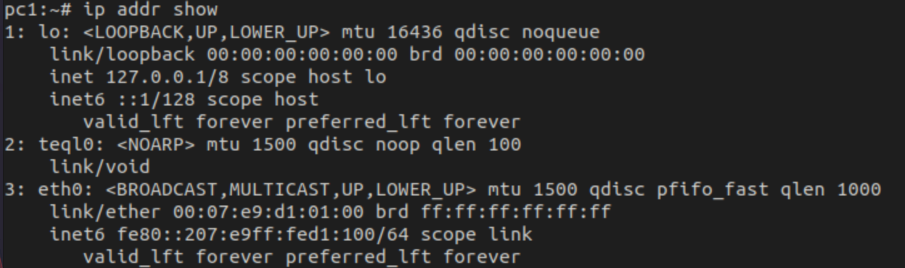
\includegraphics[width=0.4\textwidth]{ej2_3_4}&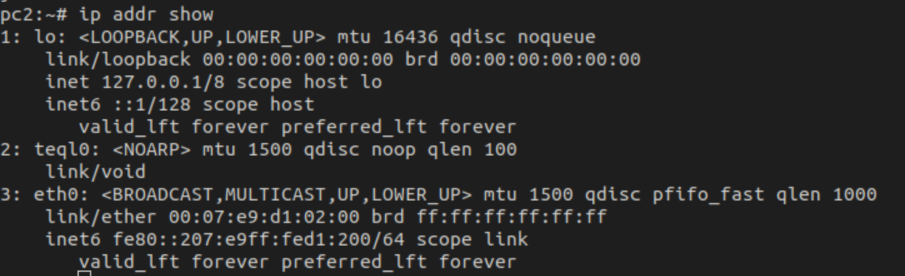
\includegraphics[width=0.4\textwidth]{ej2_4_4}
	\end{tabular}
	\item Observa en el final de la captura anterior que las máquinas siguen reintentando (cada vez con un plazo
	mayor) obtener una nueva dirección IP.
\end{enumerate}

\chapter{Renovación de concesiones}

\begin{enumerate}
	\item Vuelve a arrancar el servidor de DHCP en r1. Observa cómo pc1 y pc2 vuelven a obtener una dirección
	IP. Ten en cuenta que dicha configuración puede demorarse un rato porque los periodos de reintento de
	los DHCPDISCOVER son mayores.
	\item Arranca una nueva captura en r1-eth0 (\textcolor{blue}{dhcp-5.cap}). Arranca el resto de máquinas: pc3, pc4, pc5 y
	pc6. Cuando hayan terminado de arrancar, interrumpe la captura.
	\item Una de las máquinas habrá obtenido un periodo de concesión mucho mayor que las demás. Mirando los
	ficheros de \textit{leases} descubre qué máquina es y cuál es su periodo de concesión.\\
	\begin{center}
		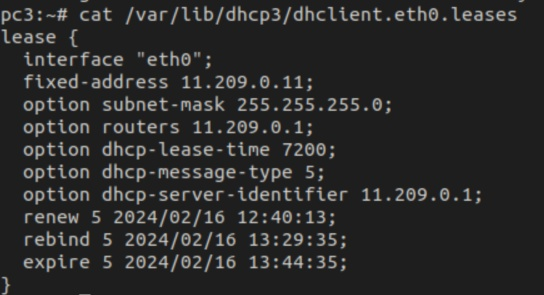
\includegraphics[width=0.6\textwidth]{ej3_5}
	\end{center}
	\item Apoyándote en el fichero de configuración de cliente de esa máquina, en el fichero de configuración del
	servidor y analizando la captura, descubre el proceso que ha llevado a que ese cliente tenga ese periodo
	de concesión. Mira cómo interpreta wireshark el periodo de concesión que solicita el cliente.\\
	
	En el fichero de configuración de pc3 se añade la opción de: \textit{send dhcp-lease-time -1;}, lo que causa que el servidor le responda con el tiempo máximo, en este caso 7200 segundos o 2 horas.\\
	Esto se puede ver en la captura de Wireshark.\\
	\begin{center}
		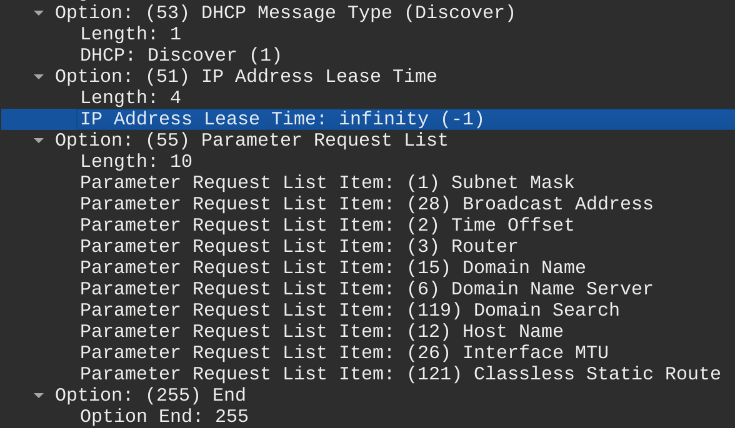
\includegraphics[width=0.6\textwidth]{ej4_5}
	\end{center}	
	\item Intenta modificar el fichero de configuración del servidor de forma que la concesión obtenida por dicho
	cliente sea de 1 día. Recuerda reiniciar el servidor tras cambiar su configuración, y reiniciar el cliente.
	Para reiniciar el cliente basta con que ejecutes en él: \textbf{/etc/init.d/networking} restart.\\
	\begin{center}
		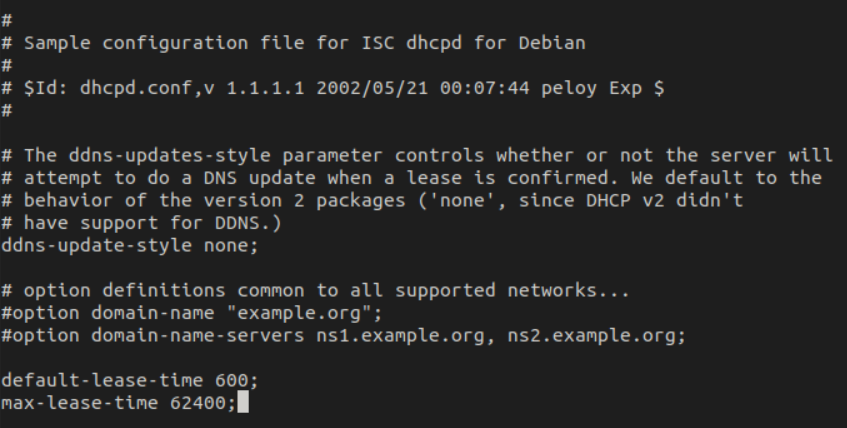
\includegraphics[width=0.6\textwidth]{ej5_1_5}
		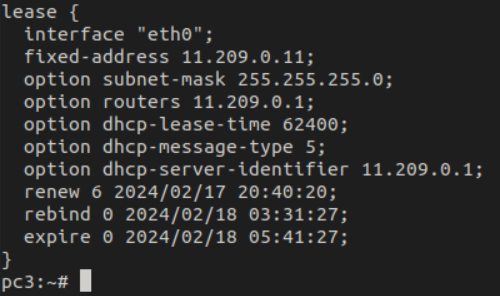
\includegraphics[width=0.6\textwidth]{ej5_2_5}
	\end{center}
	\item Intenta modificar el fichero de configuración del servidor de forma que la concesión obtenida por dicho
	cliente sea lo mayor posible.\\
	
	He modificado el tiempo en el servidor para que sea el máximo valor de un \textbf{uint32} que es 4.294.967.295, pero al enviarse el datagrama el valor máximo se reduce a 439.310.814 que es 5084 dias, 14 horas, 46 minutos, 54 segundos.
\end{enumerate}
\end{document}
